\documentclass{article}
\usepackage{authblk}
\renewcommand{\thefigure}{S\arabic{figure}}

\title{NPDR Supplementary Material}
\author[1]{Trang T. Le}
\author[2]{Bryan A. Dawkins}
\author[2,3*]{Brett A. McKinney}
\affil[1]{Department of Biostatistics, Epidemiology and Informatics,
University of Pennsylvania, Philadelphia, PA 19104}
\affil[2]{Department of Mathematics, University of Tulsa, Tulsa, OK 74104}
\affil[3]{Tandy School of Computer Science, University of Tulsa, Tulsa, OK 74104}
\renewcommand{\Authands}{ and }

\usepackage{Sweave}
\begin{document}
\Sconcordance{concordance:sup_npdr.tex:sup_npdr.Rnw:%
1 14 1 1 0 20 1}

\setkeys{Gin}{width=1\textwidth}
\maketitle
\newpage
% \section{Performance comparison between NPDR and Relief-F}

\begin{figure}[h]%figure1
\centerline{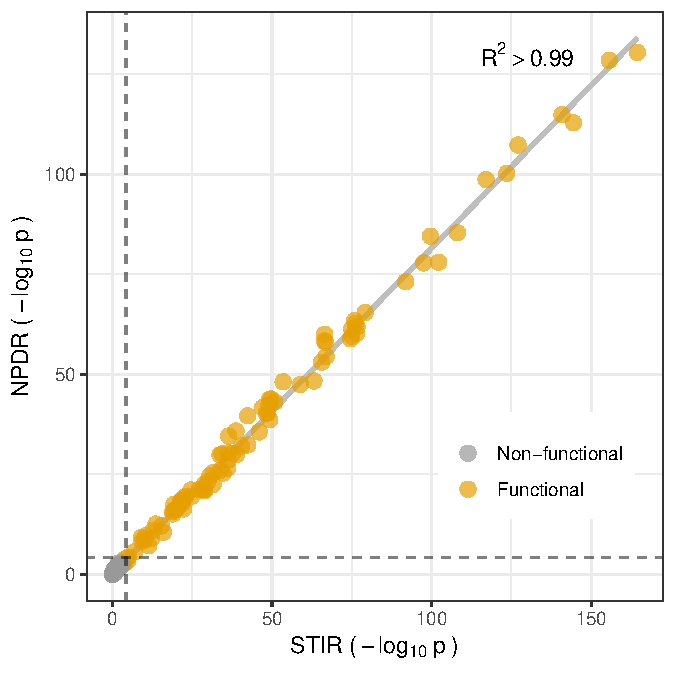
\includegraphics[]{../figs/npdr_stir_p_cc.pdf}}
\caption{Similarity between NPDR and STIR for one simulation of $m = 200$ samples and $p = 1000$ attributes. In 100 replications, $R^2$ ranges from 0.9827 to 0.9994. STIR is based on a t-test of projected distances and NPDR is based on a logistic regression of projected distances.}
\label{fig:npdr_stir}
\end{figure}

\begin{figure}[h]%figure2
\centerline{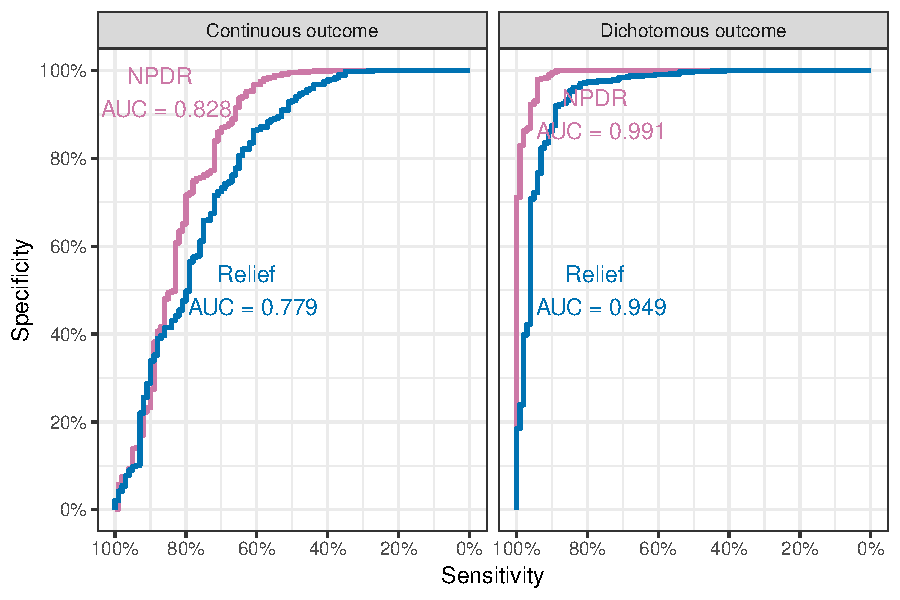
\includegraphics[]{../figs/npdr_relief_auroc.pdf}}
\caption{Receiver Operating Characteristics (ROC) curves for Relief-F and NPDR for simualted case-control data with interactions (left) and RRelief and NPDR for simulated continuous outcome data with main effects (right). Simulation uses $m = 200$ samples and $p = 1000$ attributes with 100 functional. }
\label{fig:auROC}
\end{figure}

\begin{figure}[h]%figure3
\centerline{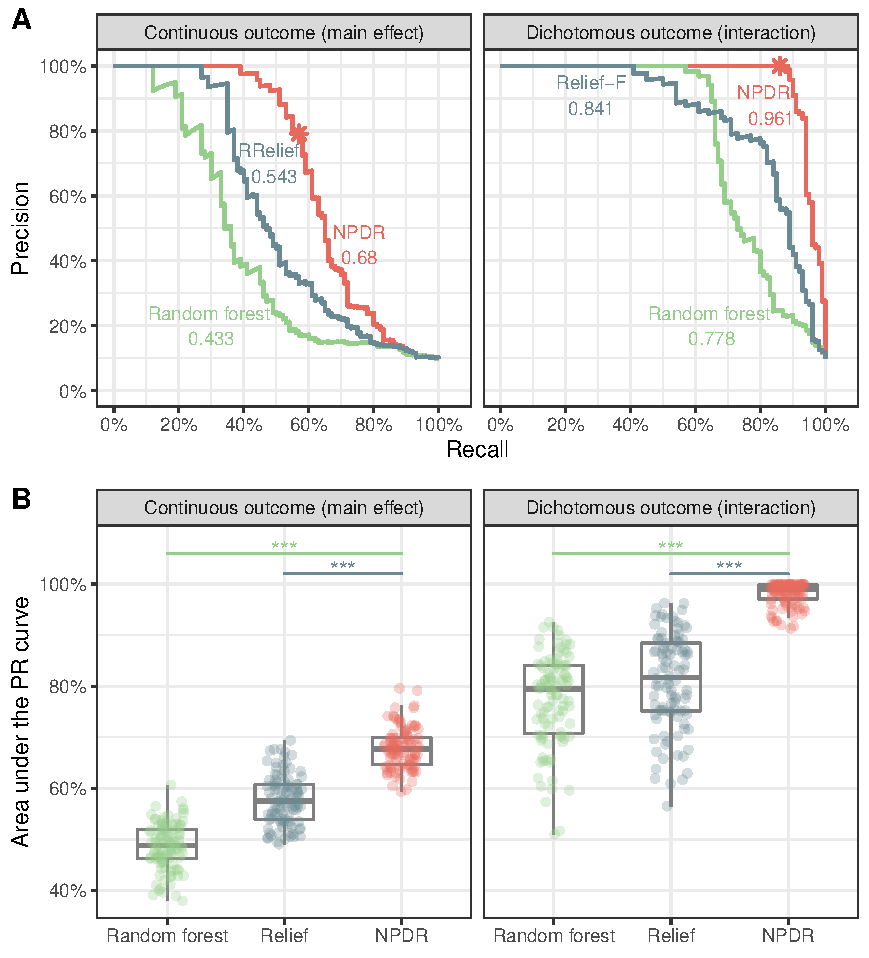
\includegraphics[]{../figs/pr_compare_100.pdf}}
\caption{NPDR and Relief comparison of area under the PRC for 100 replicate simulations of case-control (left) and continuous (right) data. All simulations use $m = 200$ samples and $p = 1000$ attributes with 100 functional. NPDR yields significantly higher auPRC.}
\label{fig:auPRC}
\end{figure}

\begin{figure}[h]%figure
\centerline{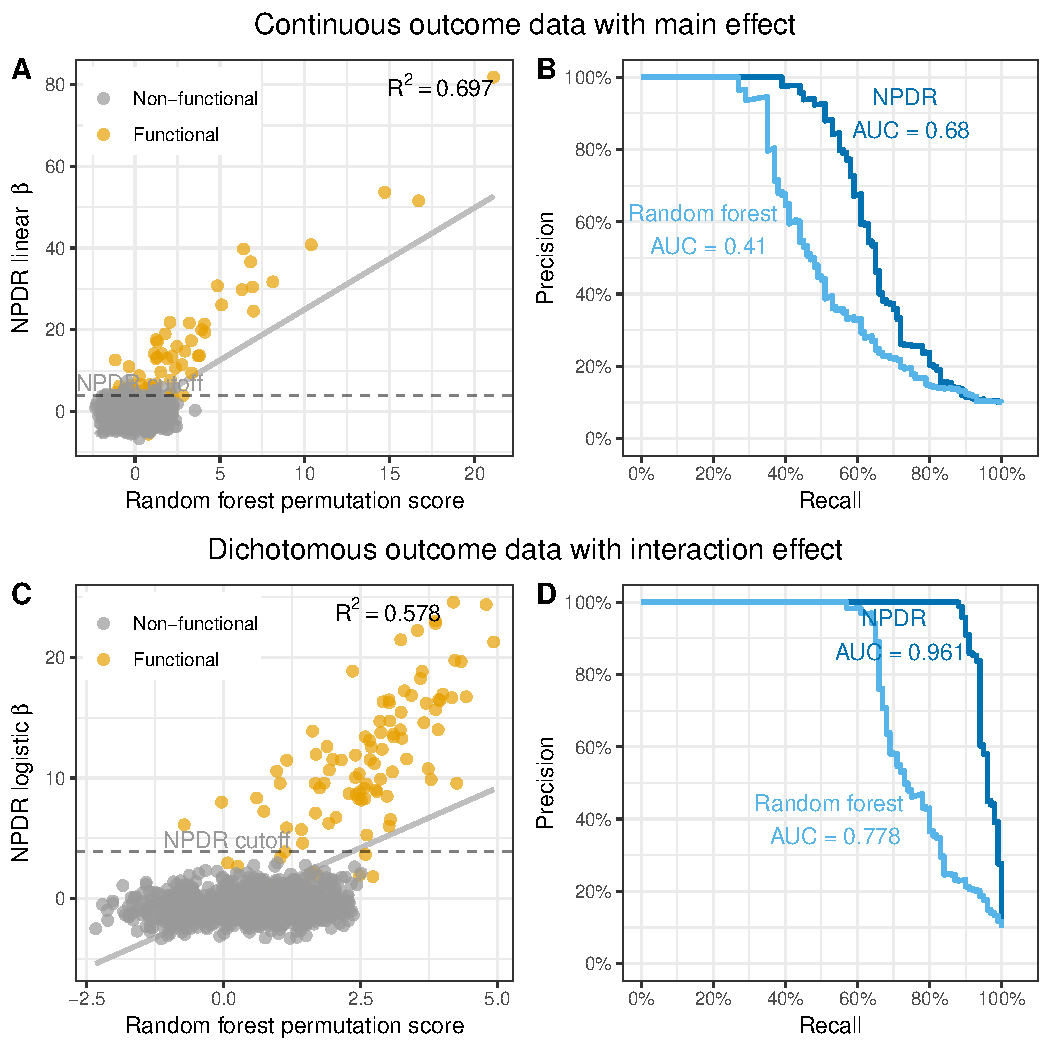
\includegraphics[]{../figs/npdr_rf.pdf}}
\caption{\textbf{Comparison of NPDR and random forest importance scores} for continuous outcome data with main effects (top row) and dichotomous outcome data with interaction effects (bottom row). Results for one replicate simulation ($m = 200$ samples and $p = 1,000$ attributes with 100 functional). For continuous outcome (A), importance scores computed by random forest permutation (percent increase in MSE) and NPDR standardized linear regression coefficient. For case-control outcome (C), scores computed by random forest permutation (mean decrease in accuracy) and NPDR standardized logistic regression coefficient. A regression line between the scores with $R^2$ is shown, and a 0.05 Bonferroni cutoff (dashed) is shown for NPDR (A and C). There is no statistical threshold for random forest, so area under the precision-recall curve (auPRC) is used to compare algorithm performance (B, D).}
\label{fig:auPRC}
\end{figure}



\begin{figure}[h]%figure
\centerline{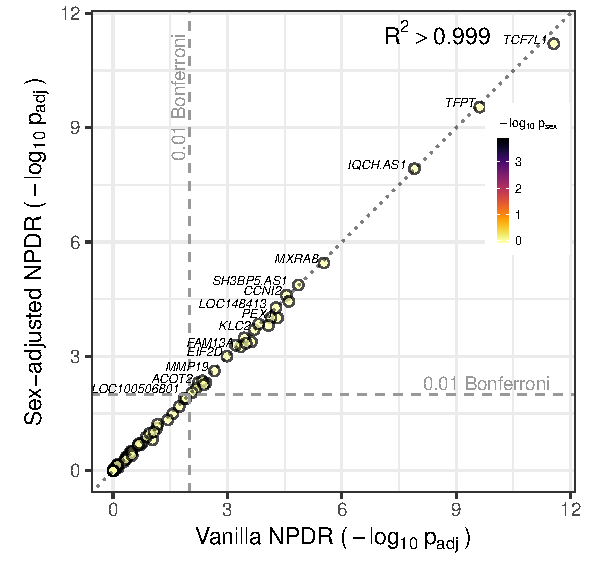
\includegraphics[]{../figs/jerzy_npdrs_mdd.pdf}}
\caption{NPDR with and without sex adjustment for analysis of MDD-associated genes in Le et al.'s RNASeq dataset. Adjustment for the sex covariate has a negligible effect on the resulting P values for each important gene because of the balanced study design. Both methods yield consistent results with STIR from previous study (Fig. 4 of Ref. \cite{stir}), not shown.}
\label{fig:jerzy_npdrs_mdd}
\end{figure}

\begin{figure}[h]%figure
\centerline{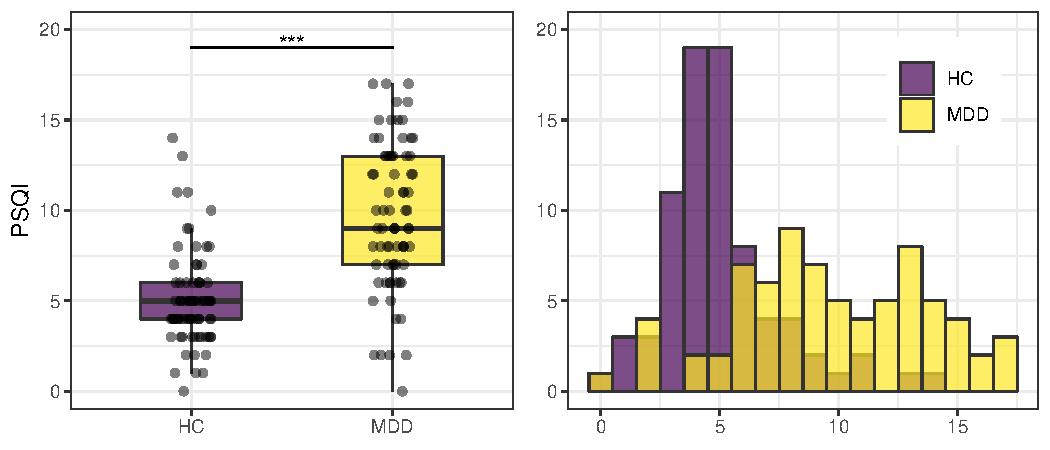
\includegraphics[]{../figs/psqi_plots.pdf}}
\caption{The distribution of the Pittsburgh Sleep Quality Index (PSQI) among individuals with and without MDD.}
\label{fig:psqi_plots}
\end{figure}


\bibliographystyle{unsrt}
\bibliography{NPDR_refs}   % name of bib file

\end{document}
